\documentclass[11pt,letter, swedish, english
]{article}
\pdfoutput=1

\usepackage{../custom_as}

\usepackage{listings} 
\usepackage[framed,numbered,autolinebreaks,useliterate]{../mcode}
\lstloadlanguages{matlab} 
\lstset{language=matlab} 

\usepackage[makeroom]{cancel}
\graphicspath{{figures/}}


\swapcommands{\Omega}{\varOmega}

%%Drar in tabell och figurtexter
%\usepackage[margin=10 pt]{caption}
%%För att lägga in 'att göra'-noteringar i texten
\usepackage{todonotes} %\todo{...}

%%För att själv bestämma marginalerna. 
\usepackage{geometry}

%%För att ändra hur rubrikerna ska formateras


%\renewcommand{\thefootnote}{\fnsymbol{footnote}}

\renewcommand{\thesubsection}{\arabic{section} (\alph{subsection})}
\renewcommand{\thesubsubsection}{\arabic{section} (\alph{subsection},\,\roman{subsubsection})}

\newcommand{\Dx}{\ensuremath{\Delta{x}}}
\newcommand{\Dt}{\ensuremath{\Delta{t}}}

\begin{document}




%%%%%%%%%%%%%%%%% vvv Inbyggd titelsida vvv %%%%%%%%%%%%%%%%%

\title{Numerical solutions to PDE's -- AMATH\,741 \\
Assignment 4}
\author{Andréas Sundström}
\date{\today}

\maketitle

%%%%%%%%%%%%%%%%% ^^^ Inbyggd titelsida ^^^ %%%%%%%%%%%%%%%%%

\section{Two characteristics for the Burgers' equation}
%\renewcommand{\thesubsection}{(\roman{subsection})}
In this problem we have two different IC's for the Burgers' equation
\begin{equation}
u_t + \frac{1}{2} (u^2)_x = 0\qcomma
-\infty<x<\infty, t>0.
\end{equation}
We already know that the characteristics for the Burgers' equation are
\begin{equation}
\dv{x}{t} = u \quad\text{constant.}
\end{equation}
This equation will be used to determine the slopes of the
characterisitcs. 
\\[11pt]
\noindent
\textbf{(i) }
The first IC is
\begin{equation}\label{eq:1_iIC}
u(x, 0) = 
\begin{cases}
-2\qcomma x<0,\\
-1\qcomma x\ge0.
\end{cases}
\end{equation}
The characteristics and solution at $t=1$ are shown in \figref{fig:1i}.

\begin{figure}
\centering
\resizebox{!}{3.6cm}{\input{figures/1i.pdf_t}}
\caption{The characteristics (left) and the solution at $t=1$ (right) 
  resulting from the IC \eqref{eq:1_iiIC}. We get rearefaction since
  the characteristics move away from each other.} 
\label{fig:1i}
\end{figure}

%\\[11pt]
\noindent
\textbf{(ii) }
The second IC is
\begin{equation}\label{eq:1_iiIC}
u(x, 0) = 
\begin{cases}
-1\qcomma x<0,\\
-2\qcomma x\ge0.
\end{cases}
\end{equation}
It is oblious that we will get a shock, so we calculate the kown shock
speed for Burgers' equation, whick is
\begin{equation}
\dot\xi = \frac{u^++u^-}{2} = -\frac{3}{2}.
\end{equation}
The characteristics and solution at $t=1$ are shown in \figref{fig:1ii}.

\begin{figure}
\centering
\resizebox{!}{3.6cm}{\input{figures/1ii.pdf_t}}
\caption{The characteristics (left) and the solution at $t=1$ (right)
  resulting from the IC \eqref{eq:1_iIC}. This time we get a shock
  since the characteristics overlap. } 
\label{fig:1ii}
\end{figure}



\section{Same as before, but different equation}
This time the governing equation is
\begin{equation}\label{eq:2_pde}
0 = u_t + \frac{1}{3} (u^3)_x = u_t + u^2u_x\qcomma
-\infty<x<\infty, t>0.
\end{equation}
To get the characteristic, $x(t)$ s.t. $u(x(t), t)$ is const., we use
\begin{equation}
0 = \dv{t} \qty[u(x(t), t)] = u_t + \dv{x}{t}u_x,
\end{equation}
which together with \eqref{eq:2_pde} leads to
\begin{equation}
\dv{x}{t} = u^2.
\end{equation}
We might as well calculate the shock speed while we're at it. Using
the Rankine-Hugoniot condition, we get
\begin{equation}
\dot\xi = \frac{f(u^+) - f(u^-) }{u^+ - u^-} 
= \frac{1}{3}\frac{(u^+)^3 - (u^-)^3}{u^+ - u^-}.
\end{equation}
From here, we just proced as in the previous problem.
\\[11pt]
\noindent
\textbf{(i) }
The first IC is the same as \eqref{eq:1_iIC}.
The characteristics and solution at $t=1$ are shown in \figref{fig:2i}.

\begin{figure}
\centering
\resizebox{!}{3.6cm}{\input{figures/2i.pdf_t}}
\caption{The characteristics (left) and the solution at $t=1$ (right)
  resulting from the IC \eqref{eq:1_iIC}. We get a shock
  since the characteristics overlap, this time the shock speed is
  $\dot\xi=7/3$. } 
\label{fig:2i}
\end{figure}

%\\[11pt]
\noindent
\textbf{(ii) }
The second IC is the same as \eqref{eq:1_iiIC}.
The characteristics and solution at $t=1$ are shown in
\figref{fig:2ii}. It is interesting to note however that since the
propagation speed from \eqref{eq:2_pde} is $u^2$, we would expect the
connecting curve between the upper and lower parts of the former
discontinuity to be parabolic. More precisely it would be a segment of
the curve $x= t\,u^2$.
\begin{figure}
\centering
\resizebox{!}{3.6cm}{\input{figures/2ii.pdf_t}}
\caption{The characteristics (left) and the solution at $t=1$ (right) 
  resulting from the IC \eqref{eq:1_iiIC}. We get rearefaction since
  the characteristics move away from each other. Note the parabolic
  shape of the connectiong curve between the upper and lower level.} 
\label{fig:2ii}
\end{figure}

\section{More modified Burgers}
\renewcommand{\thesubsection}{\arabic{section} (\alph{subsection})}
Here we begin with Burgers' equation
\begin{equation}\label{eq:3_u}
u_t + \frac{1}{2}(u^2)_x = u_t + uu_x = 0.
\end{equation}
Then we multiply both sides by $u$ and rewrite to get
\begin{equation}\label{eq:3_w}
w_t + \frac{2}{3} (w^{3/2}) = 0,
\end{equation}
where $w=u^2$.

\subsection{Show equivalence}
Here we want to show that \eqref{eq:3_w} is equivalent to
\eqref{eq:3_u} given that $u$ and $w$ are \emph{smooth} solutions to
their respective equation and that $w=u^2$.

Given that $u$ is smooth, so must $w=u^2$, so we now subsitute this
into \eqref{eq:3_w} and get
\begin{equation}
0 = (u^2)_t + \frac{2}{3} (u^{3})_x = 2u \qty[u_t+uu_x].
\end{equation}
But the expression in brackets are nothing but the LHS of
\eqref{eq:3_u}. This means that
\eqref{eq:3_u}~$\Rightarrow$~\eqref{eq:3_w}, and
\eqref{eq:3_w}~$\Rightarrow$~\eqref{eq:3_u} if $u\neq0$.

To show that $w=u^2$ also requires that their initial conditions must
satisfy $w_0=(u_0)^2$. We can look at the equations for their
characteristics
\begin{equation}
\begin{cases}
\dv{x_u}{t} = u \\
\dv{x_w}{t} = w^{1/2}.
\end{cases}
\end{equation}
We see that if we put $w=u^2$, both characteristics are going to be
the same, given $u>0$. This means that if we want $w(x(t),t) =
w_0(x(0))$ to equal the square of $u(x(t),t) = u_0(x(0))$, then
obliously $w_0 = (u_0)^2$. Or vice versa, if $w_0 = (u_0)^2$, then
it's clear from the characteristics that $w=u^2$.\footnotemark{}

\footnotetext{We also need the BC's to match according to the square
  realtion. But since we don't even know the domain, it is hard to
  specify them any further. }

\subsection{Counter example when solutions not smooth}
If the solutions aren't smooth, then we cannot safely differentiate
and expect us to get the same in the two cases. 

For instance let's use this example:
\begin{equation}
u(x, 0) = u_0(x) =
\begin{cases}
b\qcomma x<0\\
a\qcomma x\ge0,
\end{cases}
\end{equation}
where $0<a<b$. And $w(x, 0) = w_0(x) = [u_0(x)]^2$. The
Rankine-Hugoniot shock speeds for the two equations are
\begin{equation}
\begin{cases}
\dot\xi_u = \frac{1}{2}\frac{b^2-a^2}{b-a},\\
\dot\xi_w = \frac{2}{3}\frac{(b^2)^{3/2}-(a^2)^{3/2}}{b-a}.
\end{cases}
\end{equation}
Obviously
\begin{equation}
\frac{\dot\xi_u}{\dot\xi_w}=\frac{3}{4}\frac{b^2-a^2}{b^{3}-a^{3}} 
\neq1
\end{equation}
in general. 
This means that the shock will propagate with different speeds
depending on which equation is used, thus resulting in $w\neq u^2$.
 

\section{A type of advection equation with non-constant coefficients}
This time the equation in question is
\begin{equation}\label{eq:4_pde}
u_t - (1+2t)u_x = \varphi(x, t)\qcomma
-\infty<x<\infty,\; t>0.
\end{equation}

\subsection{Equation for the characteristics}
Here we first want to find the equation for the characteristic,
$x(t)$, of \eqref{eq:4_pde}. Given the definition of a characteristic
that ``it is a on which a PDE is reduced to an ODE'', we can let
\begin{equation}
\varphi = \pdv{t}\qty[u(x(t), t)] = u_t + \dv{x}{t}u_x.
\end{equation}
This together with \eqref{eq:4_pde} lets us determine an explicit
equation for the characteristics, namely
\begin{equation}\label{eq:4_char}
\dv{x}{t} = - (1+2t)
\quad\Longrightarrow\quad
x(t) = C - \qty(t + \frac{1}{2})^2,
\end{equation}
where $C$ is some constant. In words the caracteristics are parabolas,
with their openings in the negative $x$ direction and their vertexes
in the points $(C, -1/2)$. Also since $t>0$, the characteristics are
only the sections above the $x$ axis. 


\subsection{Plot of the characteristics}

To get the specific characteristic that goes through a point
$(x_0, t_0)$, we just solve the equation
\begin{equation}
x_0 = C - \qty(t_0 + \frac{1}{2})^2
\end{equation}
for $C$, and get
\begin{equation}
C_0 = x_0 + \qty(t_0 + \frac{1}{2})^2.
\end{equation}
In the special case of $(x_0, t_0) = (0, 1)$, we have $C_0 = 9/4$. A
plot of different characterisics can be found in \figref{fig:4b}.

\begin{figure}
\centering
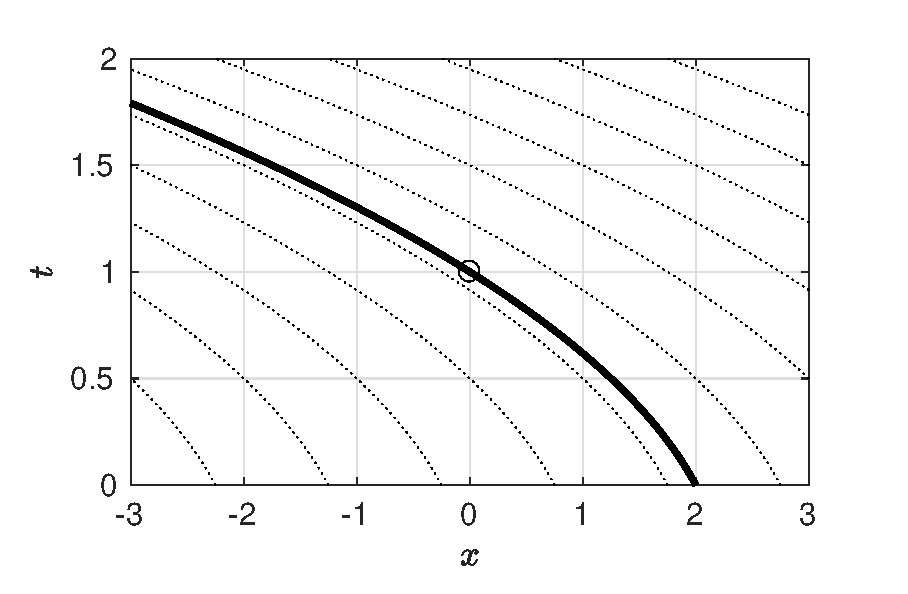
\includegraphics[width=.7\textwidth]{4b.eps}
\caption{Different characteristics of \eqref{eq:4_pde}. Especially the
  characteristic $x_0(t) = 9/4 -(t+1/2)^2$, that goes through the
  point $(x_0, t_0) = (0, 1)$, is marked out as a thicker line.} 
\label{fig:4b}
\end{figure}



\end{document}




%  LocalWords:  MFT MF Advection PDE's AMATH IC discretization MATLAB
%  LocalWords:  termwise Neumann von
